\documentclass[12pt]{article}
\usepackage{mathtools}
\usepackage{amssymb}
\usepackage{amsthm}
\usepackage{pgfplots}
\usepackage{tikz}
\usetikzlibrary{calc}
\usepackage{polski}
\usepackage[utf8]{inputenc}
\usepackage{geometry}
\usepackage{amsmath}
\usepackage{gensymb}
\usepackage{mnsymbol}
\usepackage{graphicx}
\usepackage{textgreek}
\usepackage{float}
\usepackage{caption}
\begin{document}
\newgeometry{tmargin=2cm,bmargin=2cm,lmargin=2cm,rmargin=2cm}
\tableofcontents \newpage
\section{Cel ćwiczenia}
Celem ćwiczenia było zbadanie zależności energii fotoelektronów w zależności od długości światła padającego na metal oraz wyznaczenie stałej Plancka i pracy wyjścia.
\section{Wstęp teorytyczny}
Zjawisko fotoelektryczne polega na emisji elektronów z powierzchni metalu pod wpływem padającego promieniowania elektromagnetycznego (światła widzialnego lub promieniowania ultrafioletowego). Ilość wybijanych fotoelektronów jest proporcjonalna do natężenia padającego światła. Energia kinetyczna fotoelektronów nie zależy od natężenia światła, a tylko od jego częstotliwości. Dla każdego metalu istnieje pewna częstotliwość graniczna (progowa) promieniowania, poniżej której zjawisko nie zachodzi. \newline
Zjawisko fotoelektryczne zostało wyjaśnione przez A. Einsteina, w oparciu o teorię korpuskularną światła. Założył on, że światło jest strumieniem fotonów (kwantów) o masie spoczynkowej równej zeru i energii:
\begin{center}
\Large $E=hf=\frac{hc}{\lambda}$,
\end{center}
gdzie $h$ to stała Plancka, $c$ to prędkość światła, a $\lambda$ to długość fali padającego światła. \newline
Każdy foton wybija z metalu jeden elektron. Do uwolnienia elektronu potrzebna jest praca wyjścia czyli najmniejsza energia, jaką należy dostarczyć elektronowi danego ciała, aby opuścił on ciało i stał się elektronem swobodnym. \newline
Zatem jeśli foton ma mniej energii niż wynosi praca wyjścia, nie spowoduje on emisji elektronu. Ze względu na małą wartość pracy wyjścia oraz to że dotyczy ona elektronów najczęściej używaną jednostką do jej wyrażania jest elektronowolt. \newline
Foton uderzając w elektron przekazuje mu całą swoją energię. Część tej energii zużywana jest na pracę wyjścia, reszta stanowi energię kinetyczną elektronu.
\begin{center}
\Large $E_f=hf=W+E_k$,
\end{center}
gdzie $E_f$ to energia kwantu $hf$, $W$ to praca wyjścia, a $E_k$ to energia kinetyczna elektronu. \newline
Nie wszystkie elektrony mają jednakowo dużą energię kinetyczną bo tylko część z nich dolatuje do elektrody; przy $U = 0$ prąd jest mniejszy od maksymalnego. Wreszcie przy dostatecznie dużym napięciu równym $U_h$ zwanym napięciem hamowania prąd zanika. Różnica potencjałów $U_h$ pomnożona przez ładunek elektronu $e$ jest więc miarą energii najszybszych elektronów (przy $U = U_h$ nawet najszybsze elektrony są zahamowane, nie dochodzą do elektrody). \newline
Napięcie hamujące jest niezależne od natężenia światła padającego, natomiast natężenie prądu nasycenia jest wprost proporcjonalne do natężenia światła padającego (liczba wybitych elektronów wzrasta). Napięcie hamowania $U_h$ zależy liniowo od częstotliwości padającego światła. \newpage
\noindent Maksymalną energię kinetyczną $E_{kmax}$ można zmierzyć, dobierając napięcie zewnętrzne $U=U_h$. Mierzony prąd $I$ spada wówczas do zera. W takim przypadku 
$E_{kmax}$ równe jest pracy $eU_h$. Zmierzenie wartości napięcia hamowania $U_h$ dla kilku częstotliwości światła $f$ pozwala otrzymać wykres zależności $U_h(f)$ dany teorytycznym wzorem:
\begin{center}
\Large $U_h=\frac{h}{e}f-\frac{W}{e}$
\end{center}
Nachylenie prostej $U_h(f)$ wynosi $\frac{h}{e}$, co pozwala nam wyznaczyć wartość stałej Plancka $h$. Przecięcie prostej z osią pionową stanowi zaś miarę pracy wyjścia (podanej w $eV$). \newline
Światło ma podwójną naturę. W pewnych zjawiskach ujawnia ono swoje właściwości falowe, \newline a w innych zachowuje się jak strumień cząstek, które nazywamy fotonami. Fotony nie mają masy, lecz posiadają energię. Energia jednego fotonu nosi nazwę kwantu energii. Światło jest więc równocześnie falą i strumieniem fotonów. Między wielkościami opisującymi światło jako falę, takimi jak długość i częstotliwość fali, a wielkościami opisującymi światło jako strumień fotonów, takimi jak pęd fotonu i energia fotonu, istnieją ściśle określone związki.
\begin{figure}[H]
\centering
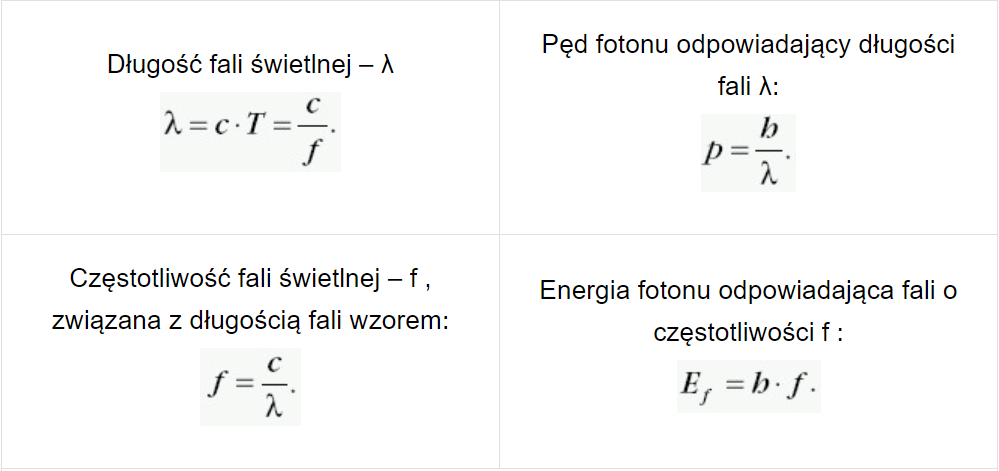
\includegraphics[width=15cm]{1}
\caption*{\textbf{Rys. 1}: Wielkości falowe i odpowiadające im wielkości korpuskularne}
\end{figure} 
\noindent Przykładem zastosowania zjawiska fotoelektrycznego jest fotokomórka, czyli element elektroniczny, którego działanie jest uzależnione od obecności światła. Przeważnie jest to bańka próżniowa, na której od strony wewnętrznej naniesiona jest warstwa metalu, czyli jedna z elektrod (jest to katoda), a wewnątrz bańki jest metalowy pręt, czyli druga z elektrod (anoda). Elementy są światłoczułe - gdy nie ma światła nie ma również przepływu prądu. Gdy w bezpośrednim kontakcie fotokomórki pojawia się wiązka światła, zapoczątkowuje ona przepływ prądu przez fotokomórkę. Przepływ jest uzależniony od natężenia światła - im jest go więcej tym swobodniej płynie prąd. \newpage
\section{Układ pomiarowy}
Przyrządy potrzebne do wykonania doświadczenia (Rys. 2): \newline
1. Żarówka \newline
2. Filtry barwne \newline
3. Fotokomórka (A - anoda, K - katoda) \newline
4. Nanoamperomierz \newline
5. Woltomierz analogowy \newline
6. Potencjometr \newline
7. Zasilacz napięcia stałego \newline
\begin{figure}[H]
\centering
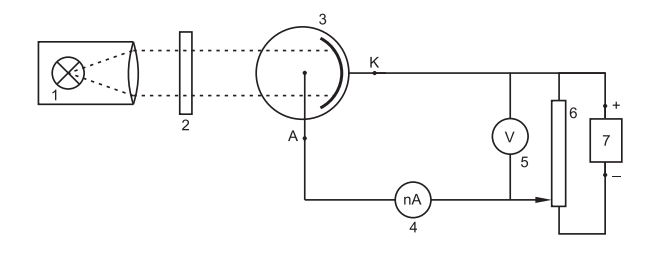
\includegraphics[width=10cm]{2}
\caption*{\textbf{Rys. 2}: Schemat układu pomiarowego do wyznaczania stałej Plancka, oznaczenia zostały opisane powyżej}
\end{figure} 
\section{Przebieg ćwiczenia}
Po zapoznaniu się z zestawem ćwiczeniowym podłączyliśmy zestaw zgodnie z instrukcją ćwiczenia. Ustawiliśmy zakres pomiarowy nanoamperomierza przez wciśnięcie klawiszy $A$ i $1\mu{A}$. Zasłoniliśmy fotokomórkę przez wysunięcie uchwytu filtru kasetki w przód. Włączyliśmy układ zasilania fotokomórki i wyzerowaliśmy nanoamperomierz odpowiednim pokrętłem potencjometru. Po ustawieniu filtru żółtego wysunęliśmy kasetkę i odczytaliśmy wskazanie nanoamperomierza. Następnie zwiększaliśmy wartość napięcia hamującego przyłożonego do elektrod fotokomórki, aż do uzyskania zerowej wartości natężenia prądu fotoelektrycznego. Odczytaliśmy wartość napięcia odcięcia $U_h$ dla światła żółtego. Powtórzyliśmy pomiar $3$ razy. Te same czynności powtórzyliśmy dla filtrów o innych barwach. Wszystkie pomiary zamieściliśmy w tabelce. \newpage
\section{Wyniki pomiarów}
\begin{figure}[H]
\centering
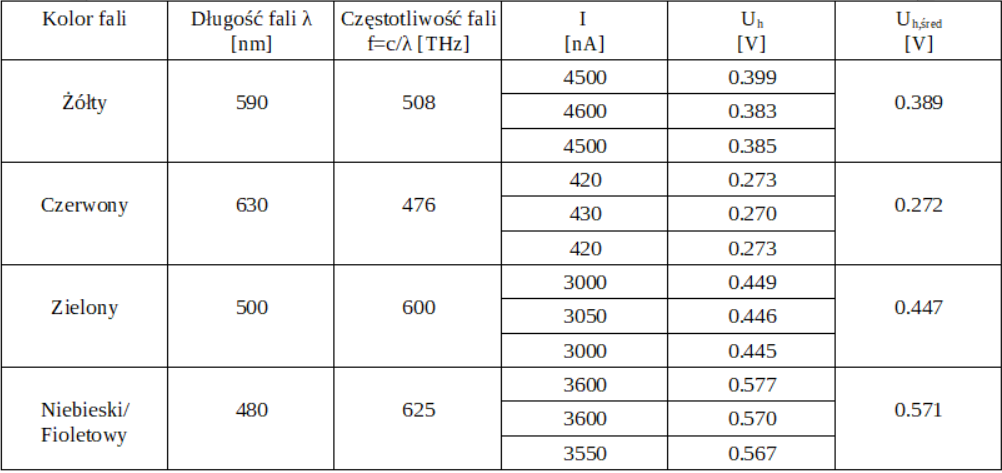
\includegraphics[width=18cm]{3}
\caption*{\textbf{Tab. 1}: Wyniki pomiarów zależności napięcia hamowania $U_h$ od częstotliwości $f$}
\end{figure} 
\begin{figure}[H]
\centering
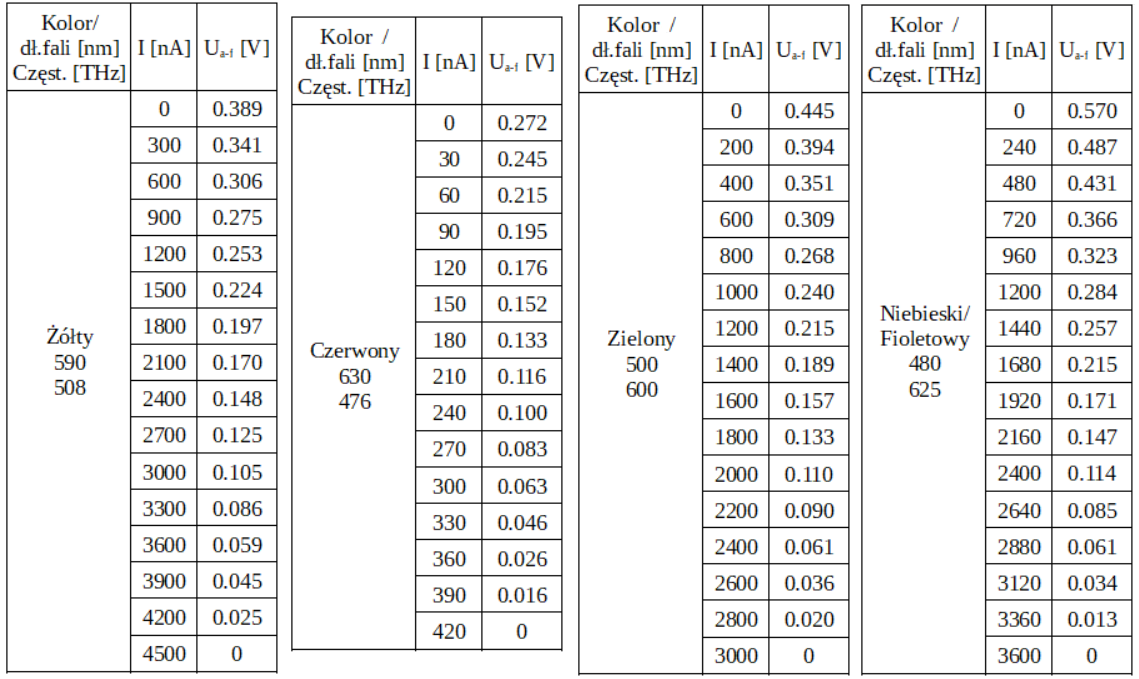
\includegraphics[width=18cm]{4}
\caption*{\textbf{Tab. 2}: Wyniki pomiarów zależności prądu fotokomówki $I$ od napięcia hamującego $U_{a-f}$}
\end{figure} 
\section{Opracowanie wyników pomiarów}
\subsection{Wykres zależności $U_h(v)$ oraz dopasowana prosta przy pomocy regresji liniowej}
\begin{center}
\begin{tikzpicture}[scale=1.5]
\begin{axis}[
title={Wykres zależności $U_h(v)$},
xlabel={Częstotliwość $f\;[THz]$},
ylabel={Napięcie hamowania $U_h\;[V]$},
legend pos=north west,
ymajorgrids=true,grid style=dashed
]

\addplot[color=black,mark=square, only marks]
coordinates {
(508,0.389)
(476,0.272)
(600,0.447)
(625,0.571)
};

\addplot [
	domain=470:630,
	samples=100,
	color=red,
] 
{0.001626044*x-0.47831435};
\end{axis}
\end{tikzpicture}
\end{center}
\subsection{Wyznaczenie stałej Plancka oraz pracy wyjścia}
Do znalezienia prostej dopasowanej do wykresu użyliśmy regresji liniowej. Wspomogliśmy się arkuszem kalkulacyjnym, który wyznaczył nam linię dopasowania:
\begin{center}
\Large $U_h=0.00163\;\frac{V}{THz}*f-0.48\;V$
\end{center}
Program wyznaczył również niepewności pomiarowe $u(a)=0.00044\;\frac{V}{THz}$ oraz $u(b)=0.24\;V$. \newline
Porównując powyższe równanie z równaniem $U_h=\frac{hf}{e}-\frac{W}{e}$ otrzymujemy, że:
\begin{center}
\Large $a=\frac{h}{e}$,   $b=-\frac{W}{e}$
\end{center}
Co po przekształceniach daje nam wzory na stałą Plancka oraz pracę wyjścia:
\begin{center}
\Large $h=ae$,   $W=-be$
\end{center} \newpage \noindent
Dla $e=1.602*10^{-19}\;C$ wartość stałej Plancka wynosi:
\begin{center}
\Large $h=ae=0.00163\;\frac{V}{THz}*1.602*10^{-19}\;C=0.00163*10^{-12}\;\frac{V}{Hz}*1.602*10^{-19}\;C=2.611*10^{-34}\;Js$
\end{center}
Wartość pracy wyjścia wynosi zaś:
\begin{center}
\Large $W=-be=0.48\;V*1.602^{-19}\;C=7.690*10^{-20}\;J=0.48\;eV$
\end{center}
\subsection{Oszacowanie niepewności pomiarowych $u(h)$ oraz $u(W)$}
Przyjęliśmy, że niepewności $u(h)$ oraz $u(W)$ związane są wyłącznie z niepewnościami odpowiednio $u(a)$ oraz $u(b)$. Zatem:
\begin{center}
\Large $\frac{u(a)}{a}\approx\frac{u(h)}{h}\;\;\;=>\;\;\;u(h)=\frac{u(a)}{a}h$
\end{center}
\begin{center}
\Large $\frac{u(b)}{b}\approx\frac{u(W)}{W}\;\;\;=>\;\;\;u(W)=\frac{u(b)}{b}W$
\end{center}
W naszym przypadku:
\begin{center}
\Large $u(h)=\frac{u(a)}{a}h=\frac{0.00044\;\frac{V}{THz}}{0.00163\;\frac{V}{THz}}*2.611*10^{-34}\;J=0.705*10^{-34}\;J$
\end{center}
\begin{center}
\Large $u(W)=\frac{u(b)}{b}W=\frac{0.24\;V}{0.48\;V}*0.480\;eV=0.24\;eV$
\end{center}
Niepewności rozszerzone (dla $k=2$) wynoszą:
\begin{center}
\Large $U(h)=2*u(h)=2*0.705*10^{-34}\;J=1.410*10^{-34}\;J$
\end{center}
\begin{center}
\Large $U(W)=2*u(W)=2*0.24\;eV=0.48\;eV$
\end{center}
\subsection{Porównanie wyznaczonej wartości stałej Plancka z wartością tabelaryczną}
Wyznaczona przez nas wartość stałej Plancka wyniosła $h=2.605*10^{-34}\;Js$ zaś wartość tabelaryczna (jak podaje instrukcja ćwiczenia) wynosi 
$h_{tab}=6.63*10^{-34}\;Js$.
\begin{center}
\Large $|h-h_{tab}|=6.63*10^{-34}\;Js-2.611*10^{-34}\;Js=4.019*10^{-34}\;Js > U(h)$
\end{center}
Tablicowa wartość stałej Plancka nie mieści się w zakresie otrzymanych przez nas wyników. \newpage
\subsection{Wykresy zależności $I(U_{a-f})$}
\begin{center}
\begin{tikzpicture}[scale=1.4]
\begin{axis}[
title={Wykres zależności $I(U_{a-f})$ dla światła żółtego},
xlabel={Napięcie $U_{a-f}\;[V]$},
ylabel={Natężenie $I\;[\mu{A}]$},
legend pos=north west,
ymajorgrids=true,grid style=dashed
]

\addplot[color=black,mark=square, only marks]
coordinates {
(0.389,0)
(0.341,0.3)
(0.306,0.6)
(0.275,0.9)
(0.253,1.2)
(0.224,1.5)
(0.197,1.8)
(0.170,2.1)
(0.148,2.4)
(0.125,2.7)
(0.105,3.0)
(0.086,3.3)
(0.059,3.6)
(0.045,3.9)
(0.025,4.2)
(0,4.5)
};
\end{axis}
\end{tikzpicture}
\begin{tikzpicture}[scale=1.4]
\begin{axis}[
title={Wykres zależności $I(U_{a-f})$ dla światła czerwonego},
xlabel={Napięcie $U_{a-f}\;[V]$},
ylabel={Natężenie $I\;[\mu{A}]$},
legend pos=north west,
ymajorgrids=true,grid style=dashed
]

\addplot[color=black,mark=square, only marks]
coordinates {
(0.272,0)
(0.245,0.03)
(0.215,0.06)
(0.195,0.09)
(0.176,0.12)
(0.152,0.15)
(0.133,0.18)
(0.116,0.21)
(0.100,0.24)
(0.083,0.27)
(0.063,0.3)
(0.046,0.33)
(0.026,0.36)
(0.016,0.39)
(0,0.42)
};
\end{axis}
\end{tikzpicture}
\begin{tikzpicture}[scale=1.4]
\begin{axis}[
title={Wykres zależności $I(U_{a-f})$ dla światła zielonego},
xlabel={Napięcie $U_{a-f}\;[V]$},
ylabel={Natężenie $I\;[\mu{A}]$},
legend pos=north west,
ymajorgrids=true,grid style=dashed
]

\addplot[color=black,mark=square, only marks]
coordinates {
(0.445,0.2)
(0.394,0.4)
(0.351,0.6)
(0.309,0.8)
(0.268,1)
(0.215,1.2)
(0.189,1.4)
(0.157,1.6)
(0.133,1.8)
(0.110,2)
(0.090,2.2)
(0.061,2.4)
(0.036,2.6)
(0.020,2.8)
(0,3)
};
\end{axis}
\end{tikzpicture}
\begin{tikzpicture}[scale=1.4]
\begin{axis}[
title={Wykres zależności $I(U_{a-f})$ dla światła niebieskiego/fioletowego},
xlabel={Napięcie $U_{a-f}\;[V]$},
ylabel={Natężenie $I\;[\mu{A}]$},
legend pos=north west,
ymajorgrids=true,grid style=dashed
]

\addplot[color=black,mark=square, only marks]
coordinates {
(0.570,0)
(0.487,0.24)
(0.431,0.48)
(0.366,0.72)
(0.323,0.96)
(0.284,1.2)
(0.257,1.44)
(0.215,1.68)
(0.171,1.92)
(0.147,2.16)
(0.114,2.4)
(0.085,2.64)
(0.061,2.88)
(0.034,3.12)
(0.013,3.36)
(0,3.6)
};
\end{axis}
\end{tikzpicture}
\end{center}
Dla każdego koloru przez zmierzone punkty można przeprowadzić gładką krzywą. Oznacza to, że $U_h$ zostało zmierzone poprawnie. \newpage
\section{Wnioski}
Zmierzona wartość stałej Plancka wynosi $h=2.611*10^{-34}\;Js$ z niepewnością pomiarową \newline $u(h)=0.705*10^{-34}\;Js$, zaś wartość pracy wyjścia wyniosła $W=0.48\;eV$ z niepewnością pomiarową $u(W)=0.24\;eV$. Różnica wartości pomiędzy zmierzoną stałą Plancka a tabelaryczną jest bardzo duża. Wartość tabelaryczna jest ok. $2.5$ razy większa od wartości zmierzonej. Jednak wykresy $I(U_{a-f})$ dla poszczególnych kolorów pokazują, że wartości zostały zmierzone poprawnie. Niedokładności naszych wyników mogą wynikać z pominięcia niepewności pomiarowych takich jak niepewność woltomierza oraz amperomierza. Innym istotnym powodem mógł być błąd spowodowany czynnikiem ludzkim. Doświadczenie pozwoliło nam zrozumieć korpuskularną teorię światła.

\end{document}